\begin{center}
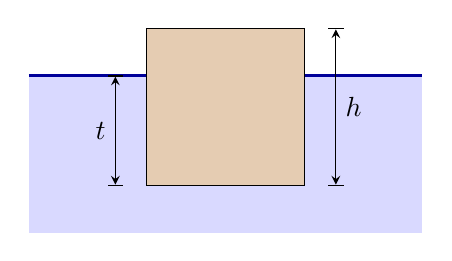
\begin{tikzpicture}[>=stealth]
 \fill[blue!15] (0,0) rectangle (5,2);
 \draw[blue!60!black, thick] (0,2) -- (5,2);
 \draw[fill=brown!40] (1.5,0.6) rectangle (3.5,2.6);
 \draw[|<->|] (3.9,0.6) -- (3.9,2.6) node[midway, right] {$h$};
 \draw[|<->|] (1.1,0.6) -- (1.1,2) node[midway, left] {$t$};
\end{tikzpicture}
\end{center}

Der Quader (Grundfläche $A$) schwimmt, wenn der Auftrieb seine Gewichtskraft aufhebt:
\begin{align}
 \rho_\text{W}\,A\,t\,g &= \rho_\text{E}\,A\,h\,g
\end{align}
Die Grundfläche fällt heraus. Mit $\rho_\text{E} = \rhoEO$ (trockenes Eichenholz, typischer Wert) und $\rho_\text{W} = \rhoWO$ (FoTaBe S.~187) ist die Eintauchtiefe
\begin{align}
 t &= \tQF \\
   &= \frac{\rhoE}{\rhoW}\cdot\hQ \\
   &= \tQ \approx \result{\tQP{-2}{2}}
\end{align}
